\documentclass[a4paper]{article}

\usepackage{graphicx}
\usepackage{multirow}
\usepackage{amsmath}
\usepackage{enumitem}
\usepackage{blindtext}
\usepackage{listings}
\usepackage{tikz}
\usetikzlibrary{automata,positioning,arrows}



\usepackage{xepersian}
\settextfont{B Roya}
\setlatintextfont{Tahoma}

\title{تمرین دوم اتوماتا}
\author{نیما بهرنگ 96100114}
\date{\today}	
\begin{document}
\maketitle
\centering{استاد خزایی}


\section*{پرسش ۱}

\pagebreak
\section*{پرسش ۲}

چون در تمام قسمت ها غیر از قسمت ث از لم تزریق استفاده می کنیم، فرض این لم را در این جا می نویسیم و در هر قسمت مستقیم به طرح روش1 ساخت طبق لم تزریق می پردازیم

 طبق لم تزریق اگر به هر ازای
\lr{n}
استیت اتوماتای محدود، وجود داشته باشد کلمه ای که تعداد حرف های آن از
\lr{n}
بیشتر باشد و
\begin{latin}
$
\forall x,y,z \in {0,1}^* : \left \{
  \begin{tabular}{ccc}
  w = xyz & \\
  |xy| $\leq$ n  & \\
  |y| $\geq$ 1 &
  \end{tabular}
\right  \} \Rightarrow \exists i \geq 0 : xy^iz \notin L
$

\end{latin}

\begin{enumerate}[label=\Alph*]

\item{)}
$w = 0^{n}1^n2^n \Rightarrow y = 0^k , |y| \geq 1 \Rightarrow xy^2z =  0^{n+k}1^n2^n \notin L$


\item{)}
$w = 0^{n}1^{2n}2^n \Rightarrow y = 0^k , |y| \geq 1 \Rightarrow xy^2z =  0^{n+k}1^{2n}2^n \notin L$


\item{)}
$w = 0^{n}1^{2n}2^n \Rightarrow y = 0^k , |y| \geq 1 \Rightarrow xy^2z =  0^{n+k}1^{2n}2^n \notin L$

\item{)}
$w = 0^{2n-1}1^{n} \Rightarrow y = 0^k, k \geq 1 , |y| \geq 1 \Rightarrow xy^2z =  0^{2n - 1+ k}1^{n} , 2n - 1 + k \geq 2*n  \Rightarrow w \notin L$

\item{)}
$w = 0^{n}110^{n} \Rightarrow y = 0^k , |y| \geq 1 \Rightarrow xy^2z =  0^{n+k}110^{n} \Rightarrow$
w is not polindrom 
$\Rightarrow w \notin L$

\item{)}
ماشینی ارائه می دهیم که هر استیت آن نشان دهنده تفاضل یک ها از صفر ها باشد و طبق فرض مسئله نباشد بیشتر از ۳ یا کمتر از -۳ شود و در ضمن با انتخاب یک یا صفر از هر استیت به استیتی متناظر تفاضل جدید می رویم
تمام استیت ها باید فاینال باشد زیرا هیچ زمانی نباید فرض مسئله نقض شود و همچنین اگر فرض مسئله رعایت شده باشد به آن معنی است که به یک حالت نهایی رفته ایم
\begin{center}
\begin{tikzpicture}[scale=0.2]
\tikzstyle{every node}+=[inner sep=0pt]
\draw [black] (15.9,-21.1) circle (3);
\draw (15.9,-21.1) node {$-3$};
\draw [black] (15.9,-21.1) circle (2.4);
\draw [black] (30.5,-7.6) circle (3);
\draw (30.5,-7.6) node {$-2$};
\draw [black] (30.5,-7.6) circle (2.4);
\draw [black] (49.7,-9.3) circle (3);
\draw (49.7,-9.3) node {$-1$};
\draw [black] (49.7,-9.3) circle (2.4);
\draw [black] (61.3,-23.4) circle (3);
\draw (61.3,-23.4) node {$0$};
\draw [black] (61.3,-23.4) circle (2.4);
\draw [black] (56.9,-42) circle (3);
\draw (56.9,-42) node {$1$};
\draw [black] (56.9,-42) circle (2.4);
\draw [black] (43.9,-49.6) circle (3);
\draw (43.9,-49.6) node {$2$};
\draw [black] (43.9,-49.6) circle (2.4);
\draw [black] (22.1,-42) circle (3);
\draw (22.1,-42) node {$3$};
\draw [black] (22.1,-42) circle (2.4);
\draw [black] (18.1,-19.06) -- (28.3,-9.64);
\fill [black] (28.3,-9.64) -- (27.37,-9.81) -- (28.05,-10.55);
\draw (24.22,-14.84) node [below] {$1$};
\draw [black] (28.3,-9.64) -- (18.1,-19.06);
\fill [black] (18.1,-19.06) -- (19.03,-18.89) -- (18.35,-18.15);
\draw (22.18,-13.86) node [above] {$0$};
\draw [black] (33.49,-7.86) -- (46.71,-9.04);
\fill [black] (46.71,-9.04) -- (45.96,-8.47) -- (45.87,-9.46);
\draw (39.95,-9.03) node [below] {$1$};
\draw [black] (51.61,-11.62) -- (59.39,-21.08);
\fill [black] (59.39,-21.08) -- (59.27,-20.15) -- (58.5,-20.78);
\draw (54.94,-17.78) node [left] {$1$};
\draw [black] (60.61,-26.32) -- (57.59,-39.08);
\fill [black] (57.59,-39.08) -- (58.26,-38.42) -- (57.29,-38.19);
\draw (58.34,-32.28) node [left] {$1$};
\draw [black] (54.31,-43.51) -- (46.49,-48.09);
\fill [black] (46.49,-48.09) -- (47.43,-48.11) -- (46.93,-47.25);
\draw (49.4,-45.3) node [above] {$1$};
\draw [black] (41.07,-48.61) -- (24.93,-42.99);
\fill [black] (24.93,-42.99) -- (25.52,-43.72) -- (25.85,-42.78);
\draw (33.91,-45.27) node [above] {$1$};
\draw [black] (24.93,-42.99) -- (41.07,-48.61);
\fill [black] (41.07,-48.61) -- (40.48,-47.88) -- (40.15,-48.82);
\draw [black] (24.93,-42.99) -- (41.07,-48.61);
\fill [black] (41.07,-48.61) -- (40.48,-47.88) -- (40.15,-48.82);
\draw (32.09,-46.33) node [below] {$0$};
\draw [black] (46.49,-48.09) -- (54.31,-43.51);
\fill [black] (54.31,-43.51) -- (53.37,-43.49) -- (53.87,-44.35);
\draw (51.4,-46.3) node [below] {$0$};
\draw [black] (57.59,-39.08) -- (60.61,-26.32);
\fill [black] (60.61,-26.32) -- (59.94,-26.98) -- (60.91,-27.21);
\draw (59.86,-33.12) node [right] {$0$};
\draw [black] (66.9,-22.4) -- (64.25,-22.87);
\draw (67.62,-22.14) node [right] {$start$};
\fill [black] (64.25,-22.87) -- (65.13,-23.22) -- (64.95,-22.24);
\draw [black] (59.39,-21.08) -- (51.61,-11.62);
\fill [black] (51.61,-11.62) -- (51.73,-12.55) -- (52.5,-11.92);
\draw (56.06,-14.92) node [right] {$0$};
\draw [black] (46.71,-9.04) -- (33.49,-7.86);
\fill [black] (33.49,-7.86) -- (34.24,-8.43) -- (34.33,-7.44);
\draw (40.25,-7.87) node [above] {$0$};
\end{tikzpicture}
\end{center}




\item{)}
$w = 0^n12^n \Rightarrow y = 0^k , k \geq 1 , |y| \geq 1 \Rightarrow xy^2z =  0^{n+k}12^n \Rightarrow (n+k) * 1 \neq n \Rightarrow w \notin L$

\end{enumerate}

\pagebreak
\section*{پرسش ۳}
\begin{enumerate}[label=\Alph*]
\item{}

$
\epsilon \in (0+01)^*
$\\
$
\epsilon \notin 00^*1*
$

\item{}
$
\epsilon \in (0+1)^*(11+0+\epsilon)^*
$\\
$
\epsilon \notin (0+1)^*11(0 + 1)*
$

\item{}
$
1 \in (1 + 10 + 11 + 1)^*
$\\
$
1 \notin (111 + 110 + 101 + 011 + 010 + 0)^*
$

\item{}
برابرند زیرا در زبان هر جفتشان هر کدام از
\lr{00, 01, 10, 11}
به دلخواه می تواند باشد
همچنین دی اف ای ضربیشان نیز تهی است زیرا هر حالت دی اف ای شان می توان یکی از 
\lr{00, 01, 10, 11}
را انتخاب کرد و برای هر دو امکان پذیر است و بعد از هر انتخاب نیز به حالتی نهایی می روند



\end{enumerate}

\pagebreak

\section*{پرسش ۴}
\begin{enumerate}[label=\Alph*]
\item{)}
 \begin{latin}
\begin{center}
 \begin{tabular}{|c || c | c | c | c | c | c|} 
 \hline
 & $ q_0$ & $q_1$ &$ q_2$ & $q_3$ &$ q_4$ & $q_5$ \\ [0.5ex] 
 \hline
$ q_0$ &  & x  &  & x & & x\\ 
 \hline
$ q_1$ & x &  & x &  & x & x\\ 
 \hline
$ q_2$ &  & x & & x & & x\\ 
 \hline
$ q_3$ & x  &  & x &  & x & x\\ 
 \hline
$ q_4$ &  & x & & x & & x\\ 
 \hline
$ q_5$ & x & x & x & x & x &\\ 
 \hline
\end{tabular}
\end{center}

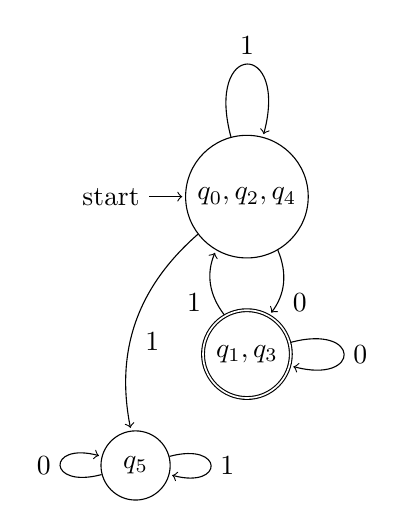
\begin{tikzpicture}[shorten >=1pt,node distance=2cm,on grid,auto] 
   \node[state,initial] (q0)   {$q_0, q_2, q_4$};
   \node[state,accepting] (q1) [below=of q0] {$q_1, q_3$};
   \node[state] (q5) [below left of= q1] {$q_5$}; 
    \path[->] 
(q0) edge  [bend left]node {0} (q1)
	edge [loop above]node{1}()
edge  [bend right]node {1} (q5)
(q1) edge  [bend left] node{1} (q0)
	edge [loop right]node{0}()
(q5) edge  [loop left]node{0}()
	edge [loop right]node{1}();
\end{tikzpicture}

\end{latin}

\item{)}
 \begin{latin}
\begin{center}
 \begin{tabular}{|c || c | c | c | c | c | c | c|} 
 \hline
 & $ q_0$ & $q_1$ &$ q_2$ & $q_3$ &$ q_4$ & $q_5$  & $q_6$ \\ [0.5ex] 
 \hline
$ q_0$ &  & x &  & x & & x & x\\ 
 \hline
$ q_1$ & x &  & x & x & x & x & x\\ 
 \hline
$ q_2$ &  & x & & x & & x &x\\ 
 \hline
$ q_3$ & x  & x  & x &  & x & &\\ 
 \hline
$ q_4$ &  & x & & x & & x &x\\ 
 \hline
$ q_5$ & x & x & x &  & x & &\\ 
 \hline
$q_6$  & x & x & x & & x & &\\ 
 \hline
\end{tabular}
\end{center}

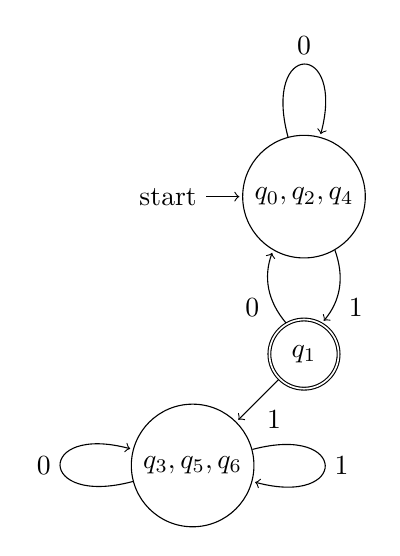
\begin{tikzpicture}[shorten >=1pt,node distance=2cm,on grid,auto] 
   \node[state,initial] (q0)   {$q_0, q_2, q_4$};
   \node[state,accepting] (q1) [below=of q0] {$q_1$};
   \node[state] (q3) [below left of= q1] {$q_3,q_5,q_6$}; 
    \path[->] 
(q0) edge  [bend left]node {1} (q1)
	edge [loop above]node{0}()
(q1) edge  [bend left] node{0} (q0)
	edge node{1}(q3)
(q3) edge  [loop left]node{0}()
	edge [loop right]node{1}();
\end{tikzpicture}

\end{latin}


\end{enumerate}

\pagebreak

\section*{پرسش ۵}
\begin{enumerate}[label=\Alph*]
\item{)}
اگر  رشته های
\lr{$0^k1, k \geq 1$}
را در نظر بگیریم، دارای خاصیت گفته شده هستند،زیرا 
هر دو عضو آن را که بگیری و متفاوت باشند مثلا
\lr{$0^n1, 0^m1, n \neq m$}
تنها رشته ای که به هرکدام از آنها می تواند اضافه شود و 
یک رشته عضو زبان بسازد رشته
\lr{$1^{k-1}$}
است که همواره به ازای هر دو عضو متفاوت و یکتاست پس یک مجموعه مورد نظر است که نامتناهی هم هست :)
\end{enumerate}
\pagebreak

\section*{پرسش ۶}

	\lstset{ basicstyle=\footnotesize\tt, % the size of the fonts that are used for the code breakatwhitespace=false, % sets if automatic breaks should only happen at whitespace breaklines=true, % sets automatic line breaking 
	captionpos=b, % sets the caption-position to bottom 
	extendedchars=true, % lets you use non-ASCII characters; for 8-bits encodings only, does not work with UTF-8 
	frame=single, % adds a frame around the code 
	language=Java, % the language of the code 
	keywordstyle=\bf, 
	showspaces=false, % show spaces everywhere adding particular underscores; it overrides 'showstringspaces' showstringspaces=false, % underline spaces within strings only 
	showtabs=false, % show tabs within strings adding particular underscores 
tabsize=2 % sets default tabsize to 2 spaces 
}
\begin{latin}
\begin{lstlisting}
<pair<char, int>> reverseAdj[n][k] \\ reverse edges in automata
\\ like if there was Q (a)-> P now : P (a)-> Q
vector<int> finals;
boolean isfinal[n];
int start;
boolean difftable[n][n]


void notfinal(int p, int q){
	difftable[p][q] = difftalbe[q][p] = true;
	for(int i = 0; i < k; i++){
		p2 = reverseAdj[p][i];
		q2 = reverseAdj[q][i];
		if(!difftable[p2][q2])
			notfinal[p2][q2];
	}
}


int main(){
	for(int i = 0; i < finals.size(); i++)
		isfinal[finals[i]] = true;
	for(int i = 0; i < finals.size(); i++)
		for(int j = 0; j < n; j++)
			if(!final[j] && !difftable[final[i]][j])
				notfinal(final[i], j)
}
\end{lstlisting}
\end{latin}
الگوریتم گفته شده همانطور که در کلاس گفته شد بر اساس اینکه هر فاینال با هر غیرفاینال، دو استیت متمایزند، در الگوریتم ما نیز همینگونه شروع می کند و به صورت بازگشتی روی قبلی ها اجرا می شود
\\
اوردر برنامه برابر
\lr{N + O(notfinal())}
است که تعداد دفعاتی که تابغ ما صدا می شود برابر مربع تعداد استیت هاست زیرا هر زوج مرتب تنها حداکثر یک بار صدا زده می شود و آن هم وقتی است که زوج مرتب دیگری که برای اولین بار صدا شده اند، با یکی از حروف زبان به این استیت آمده باشند، و سپس این زوج علامتشان زده می شود و هیچ بار دیگری تابع به ازای آنها صدا نمی شود پس تابع ما حداکثر به تعداد مربع استیت ها می تواند صدا شود\\
پس اوردر برنامه همان مربع استیت است.
\pagebreak

\section*{پرسش ۷}
چون هر زبان منظم یک عبارت منظم دارد و طبق گفته های جزوه ۷ استاد می توان هر یک از عملیات الحاق و احتماع و بستار را با یک 
\lr{$\epsilon-nfa$}
که تنها یک استیت فاینال دارد ساخت پس هر زبان منظم نیز یک
\lr{$\epsilon-nfa$}
با تنها یک استیت پایان دارد
\pagebreak
\section*{پرسش۸}
\pagebreak
\section*{پرسش۹}
\end{document}